\chapter{Analysis}

The analysis is a very important part of the whole project. It helps us to understand what is excepted from the system and how we will try to fulfil these expectations. There are many methodologies in area of software engineering but you have to do the analysis before you start to write the code no matter which methodology you choose. The analysis doesn't have to be big (especially in an agile methodology) but it has to be there.

In this chapter there is analysis of desired functionality, used frameworks and development environment. The most important part is the analysis of desired functionality because it helps to understand what is and what is not excepted from this project. The analysis of used frameworks is based on desired functionality because used framework has to be able to help with its realisation.

\section{Desired Functionality}

There are a lot of applications that provides the class modeling. Basic appearance is mostly common. There is a space where the model is shown (this space will be called workspace) and some toolbox where user can choose the tool he wants.

The application that inspired me most was Enterprise Architect from Sparx Systems \cite{sparxsystemsweb} company. This application does not provide only class modeling functionality. It is a CASE\footnote{CASE - Computer Aided Software/System Engineering} system which is used for purposes of analysis and implementation. The Enterprise Architect provides all UML diagrams (Class diagram, Activity diagram, Use Case diagram, Sequence diagram, etc.) creation and much more. But only the Class diagram is important for this project because it is what this thesis deals with. The class modeling in Enterprise Architect has a lot of functionality that cannot be created during a one bachelor thesis. Thus, it has to be decided which functionality will be implemented and which will not.

Every class diagram modeller has to be able to depict the basic elements of the class diagram as were described in section \ref{section:classDiagramDescription}. Existing modellers provides another functionality like information about complexities of single classes, their constraints, statuses, requirements, notes and many others. It is a lot of functionality that can not be created during a one bachelor project but it can be implemented in a related project.

A feature that is not a common one and is implemented in the Indepmod Class Notation Modeller is an annotation list of classes, methods and attributes. Annotations are used in the Java programming language from version 1.5 and in the C\# programming language. Annotations are form of metadata which are stored in the source code. Alternative to annotations are configuration files (very often of XML type) that hold these information. These metadata are often used by frameworks. An example can be the JPA\footnote{JPA - Java Persistence API} framework of Java EE\footnote{Java EE - Java Enterprise Edition} that uses these metadata for the definition of object relation mapping (ORM)\footnote{Object Relation Mapping - a technique that maps objects from object oriented system into tables from relation database}. In a former version of java, these metadata were stored in XML configuration files. When there was a lot of classes to be configured, these configuration files were very large and confusing. On the other hand, annotations allow to specify these configurations inside the classes. This means that if you want to see or edit a class configuration, you don't have to search it in a file with maybe hundreds or thousands lines. Instead, you will open a desired class and find these information right there.

\subsection{Class Diagram Data Model}

\begin{figure}[!ht]
\begin{center}
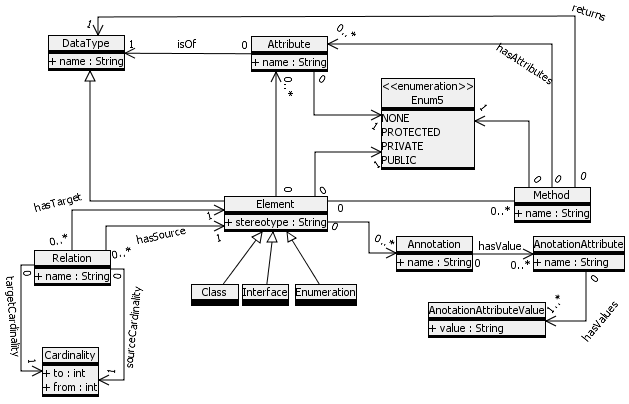
\includegraphics[scale=1]{img/classDiagramMetamodel.png}
\caption{Class Diagram Metamodel}
\label{f-classDiagramMetamodel}
\end{center}
\end{figure}

Figure \ref{f-classDiagramMetamodel} shows the data model of the class diagram that Indepmod Class Notation uses. From this data model you can see what the Indepmod Class Notation can and what it can not. Main building block of whole class diagram is an Element. The Element can be either a Class or an Interface or an Enumeration. Every Element has a visibility, a stereotype (which can be empty) and a name. Each Element defines a data type identified by its name. In addition to the stereotype and the name, the Element has also the list of annotations, attributes and methods.

An Attribute has a name, a visibility and represents a data type. This data type can be the data type of an Element that we have already created or it can be another else data type (like String or int data type in Java). The Attribute can also have several (or none) Annotations. A Method is also defined by a name and has a visibility. The Attributes owned by the Method represents the parameters and the data type represents what the method returns. An Annotation has a name and can have several Annotation Attributes. Each Annotation Attribute has the name and a list of values.

\subsection{Model Type}

The Indepmod Class Notation Plugin will allow to create two types of class model. The first one is a standard Class model which has been already described in the section \ref{section:classDiagramDescription}. The second one is a business model. The selection of desired diagram in the application type will be done when user creates a new diagram. 

The purpose of the business model has been also described in the section \ref{section:classDiagramDescription}. Business model does not use all elements of the class model. It uses classes, its attributes and relations between classes. A class represents an entity from the problem domain. An attribute describes a property of the entity and a relation represents exactly what its name says - the relation between entities. An example of the business model can be the Figure \ref{f-classDiagramMetamodel}, which describes the problem domain of the class model.

\subsection{Diagram data sharing}

The Indepmod Class Diagram Plugin will be able to provide its diagram data to another Netbean's plugin. It means that there could be a plugin which will be able to e.g. generate a code according to the model or create an report. This will be done by some public API\footnote{API - Application Programming Interface} which will be provided by this application. This API will provide the type of the diagram (class or business diagram), the information about elements of the diagram and the picture of the diagram. The picture can be used by another plugin for example for a report. Concrete implementation of the API will be described in the Architecture chapter, concrete in the section \ref{section:classModelAPI}.

\section{Used Frameworks}

\subsection{Netbeans API}
\label{section:netbeansAPI}

All desktop applications have several common things. They use for example windows, menus (file, edit, etc.), docking panels, help system, online update system, etc. This functionality can be created over and over again for each new desktop application but it takes a lot of time and effort to create it. And this is the reason why the frameworks are used. Advantage is that a developer (or a group of developers) creates and updates the framework that solves certain problem. Another developer can then use this framework so he does not have to implement it again. If the developer solved the problem himself, he would either create not so robust solution or spend a lot of time (maybe years) to create it.

The Netbeans platform is an open source application framework based on well known Swing Technology. It can be used to simplify the desktop application development by providing many techniques and design patterns. The Netbeans platform gives the developer a tool to create a robust desktop application much faster and better. Thus, the developer can focus on the application's business logic creation instead of dealing with the work that has been already done.

Basic concept of the Netbeans API is that the application can be divided into several loosely coupled modules. This is very useful especially when the application starts to be complex. Netbeans API uses a virtual filesystem (hierarchical structure of directories and files), also called as central registry, for its configuration. Every module which is deployed into the application can add some information into this virtual filesystem and thus it can add some functionality. This is described later in the section \ref{section:toolChooserModule}.



The Netbeans platform can be used either to create the whole desktop application or to create a plugin for an existing one. Both whole applications and plugins can be consisted of several (or of many) independent modules. For this project I chose the creation of a plugin. The Netbeans platform provides a lot of functionality and if you want to know more about it, please take look at \cite{netbeans6.9DevGuide}.

\subsection{JGraph}
\label{section:JGraph}

JGraph is an opensource graph visualisation library which is based on Java Swing technology. It gives the developer great means to create a generic diagram, which is consisted of nodes and edges. JGraph provides several prefabricated components for graph nodes shapes or for edges shapes that connect these nodes. Of course, there is the possibility to create your own shapes too.

Except the diagram visualisation, JGraph provides some other functionality like zooming of the drawing area, undo/redo support, drag\&drop of nodes and edges and many other. This framework will be used for visualisation of the class diagram. More information about this framework can be found in \cite{jgraphmanual}.

\section{Environment}

Because this thesis is about the Netbeans plugin creation and Netbeans platform is based on the Java language, there wasn't any other option than use the Java language. But it is not bad at all. Java is widely used object oriented programming language and thanks to its portability, the application can run on a lot of operating systems like Windows, Linux and so on.

As a programming enviroment I use the Netbeans IDE. The Netbeans IDE is the best choice because it is created on the same platform as the plugin. Netbeans IDE provides the full support (Wizards, etc.) for the Netbeans plugin (or module and whole applications based on this platform) creation. The Netbeans platform is described in section \ref{section:netbeansAPI}.
